\chapter{Assoziationsdatenbank und API}
Das Ziel von TIMA ist das Erstellen einer Datenbank, in denen Assoziation gespeichert werden. Daher liegt ein Schwerpunkt unserer Arbeit darin, diese zu Erstellen und zu Befüllen. Die Datenbank ist direkt verknüpft mit einem Webfrontend, das durch die Bereitstellung einer umfassenden API der Hauptanlaufpunkt für die Nutzer und die Applikationen ist.

In diesem Kapitel werden das Backend der Webseite und die Datenbank näher beschrieben. Dabei wird genauer auf Designentscheidungen eingegangen, die zum Aufbau der einzelnen Datenbankbestandteile geführt haben.

\section{Backend und Datenbank}
Für das Backend der Website haben wir uns für Django als grundlegende Bibliothek entschieden. Bei Django handelt es sich um ein in Python geschriebenes Webframework, das dem Model-View-Controller-Schema folgt. Django bietet unter anderem einen sehr komplexen objektrelationalen Mapper, der es ermöglicht auch komplexe Objektstrukturen abzubilden ohne die verwendete Datenbank explizit zu kennen. Neben allen notwendigen Funktionen gewährleistet Django zusätzlich also gute Wiederverwendbarkeit und wurde deshalb für das Erstellen des Backends genutzt.

\subsection{Datenmodell}
In \hyperref[fig:uml]{Abbildung \ref*{fig:uml}} ist das komplette Datenmodell von TIMA dargestellt. Das Modul \code{associations.models} spielt dabei die Schlüsselrolle. Hier werden die grundlegenden Daten für die Assoziationsdatenbank gespeichert: die Worte und deren Verknüpfungen.

\begin{figure}
	\centering
	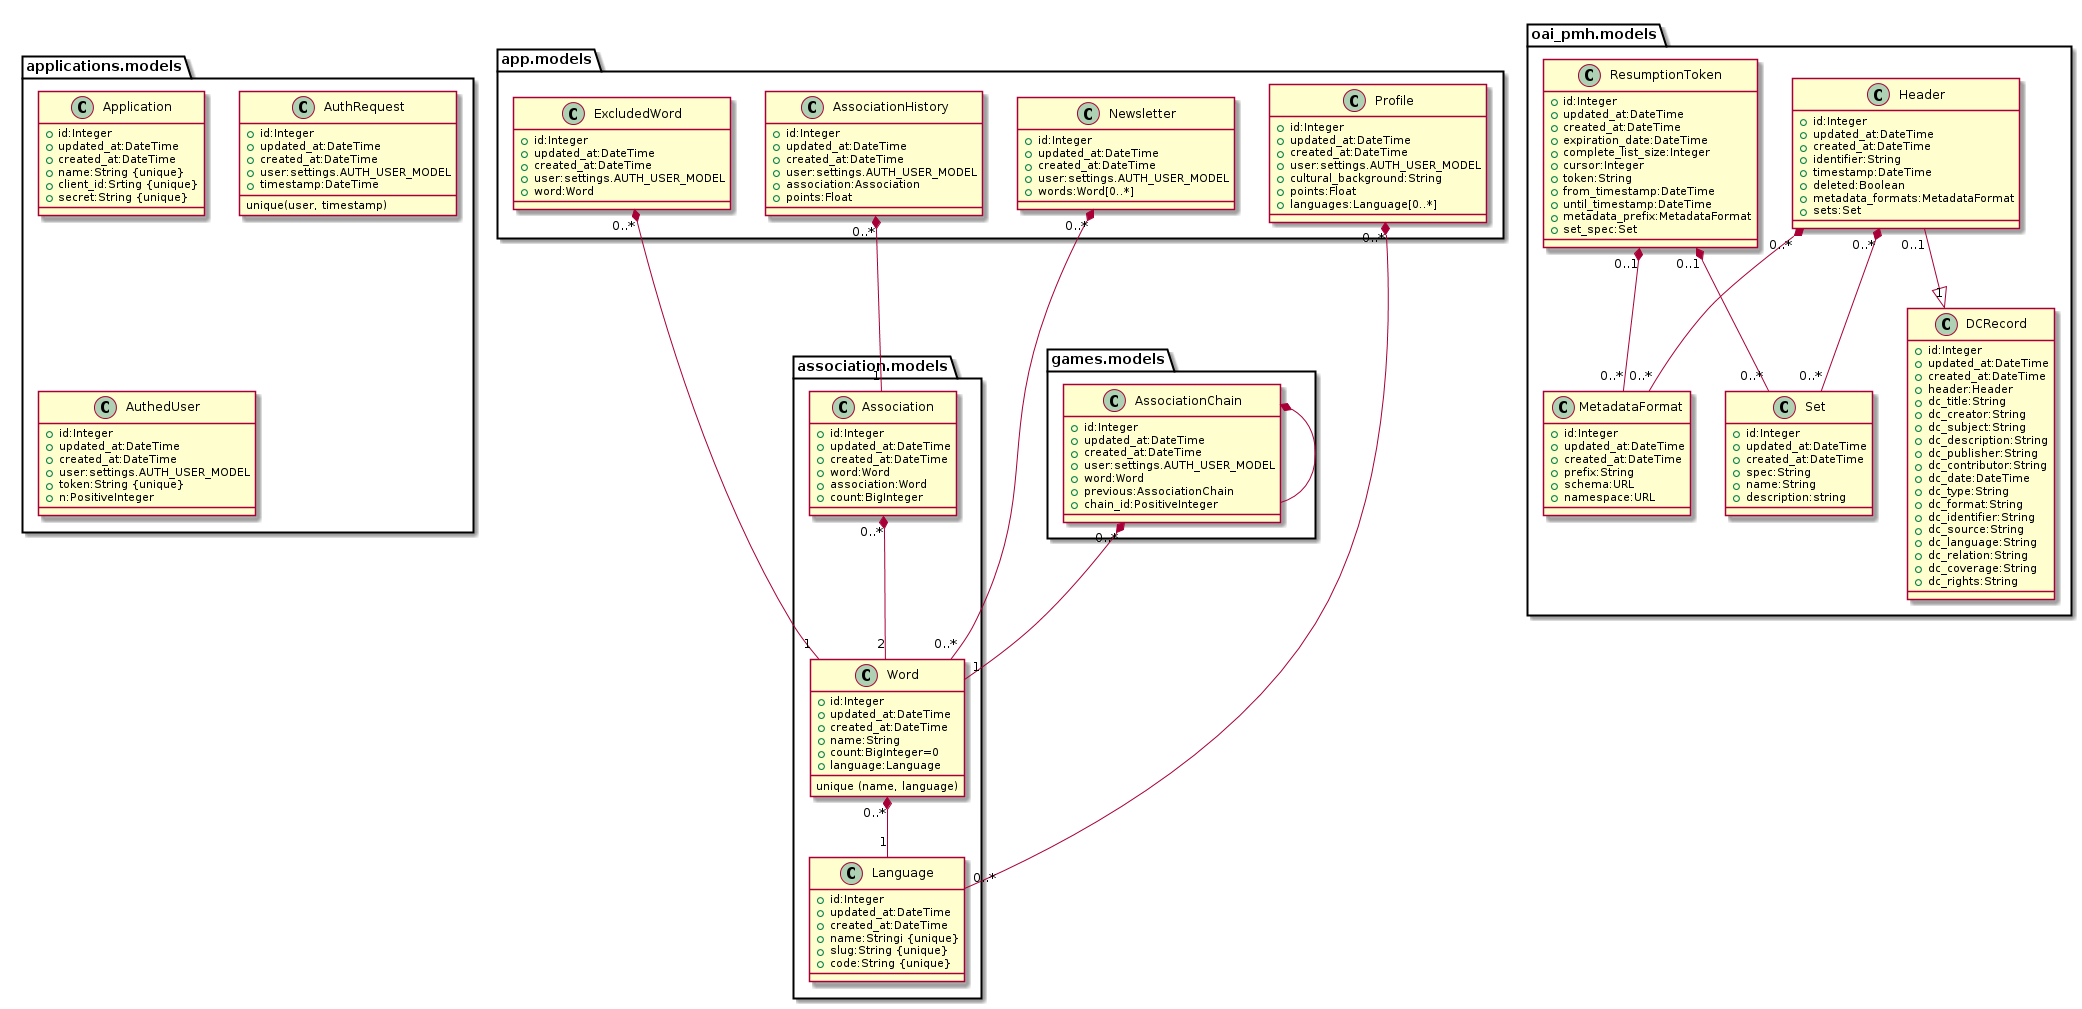
\includegraphics[width=\textwidth]{images/uml.png}
	\caption{UML des TIMA Datenmodells}
	\label{fig:uml}
\end{figure}

Das Modell \code{Word} speichert einzelne Wörter und das Modell \code{Association} die Assoziationen zwischen diesen Wörtern. Für jedes Wort wird gespeichert, wie oft für dieses nach einer Assoziation gefragt wurde. In ähnlicher Weise besitzt auch jede Assoziation in der Datenbank eine Häufigkeit, die angibt wie oft die Assoziation von Nutzern gegeben wurde.

Um eine Unterscheidung zwischen verschiedenen Sprachen zu ermöglichen, repräsentiert das Modell \code{Language} die verfügbaren Sprachen. Existiert ein Wort in mehreren Sprachen oder wird in verschiedenen Sprachen genutzt, hat es für jede Sprache einen eigenen Eintrag.

\paragraph{} Das Modul \code{games.models} enthält Modelle die für die verschiedenen Spiele wichtig sind. Dies ist im Moment nur das Spiel AssoziationsKette (vgl. \hyperref[sec:games]{Abschnitt \ref*{sec:games}}), hierfür werden in dem Modell \code{AssociationChain} die letzte beziehungsweise aktuelle Assoziationskette eines Nutzers gespeichert. Diese wird beim Start eines neuen Spieles gelöscht.

\paragraph{} Um grundlegende Funktionen des Nutzermanagements zu ermöglichen, wurden das Modul \code{app.models} eingeführt. Das Modell \code{Profile} speichert grundlegende Informationen zu jedem Nutzer, zum Beispiel die Punktzahl und die Sprachen, für die ein Nutzer assoziiert hat. Diese Daten werden in einem Ranglistensystem genutzt, das die Nutzer motivieren soll, sich gegenseitig zu messen. In dem Modell \code{AssociationHistory} wird die gesamte Assoziationsgeschichte eines Nutzers gespeichert, mit den jeweils für eine Assoziation erhaltenen Punkte. Somit können im Falle eines Missbrauchs die gegebenen Assoziationen aus der Datenbank gelöscht werden und dem Nutzer die Punkte entzogen werden.
Das Modell \code{ExcludeWord} enthält für jeden Nutzer die Wörter, die er innerhalb der letzten sieben Tage übersprungen hat (vgl. \hyperref[subsec:excludewords]{Abschnitt \ref*{subsec:excludewords}}). Das letzte Modell in diesem Modul speichert für jeden Nutzer welche Worte er in seinem Newsletter empfangen möchte.

\paragraph{} Für die Kommunikation zwischen der Applikation und dem Backend, insbesondere der Authentifizierung der Schreibzugriffe auf die Datenbank (vgl. \hyperref[sec:api]{Abschnitt \ref*{sec:api}}) dient das Modul \code{applications.models}. Das Modell \code{Applikation} speichert die Applikationen, mit denen es möglich ist sich zu authentifiziert, mit den nötigen Daten für die Authentifizierung (vgl. \hyperref[subsec:authentifizierte_anfragen]{Abschnitt \ref*{subsec:authentifizierte_anfragen}}). Die beiden anderen Modelle dieses Moduls \code{AuthRequest} und \code{AuthedUser} speichern die nötigen Information für einen Nutzer der sich authentifizieren möchte oder sich bereits authentifiziert hat. Durch dieses Modul wird also gewährleistet, dass nur Nutzer auf die Datenbank zugreifen können, die eine von uns erlaubte Anwendung nutzen.

\paragraph{} Das letzte Modul und die beinhalteten Modell sind für OAI-PMH erforderlich, näheres dazu in \hyperref[sec:oai-pmh]{Abschnitt \ref*{sec:oai-pmh}}.


\section{API}\label{sec:api}
Damit verschiedene Applikationen mit der TIMA Datenbank kommunizieren können, haben
wir uns entschieden eine umfangreiche API zu implementieren. Diese lässt sich
grob in drei Teile gliedern. Erstens gibt es die Anfragen, die keiner
Authentifizierung bedürfen, zweitens jene die eine Authentifizierung erfordern und
drittens eine OAI-PMH Schnittstelle.

Bis auf die OAI-PMH Schnittstelle, die XML zurück gibt, werden immer JSON-Objekte zurückgegeben. Jedes dieser JSON-Objekte enthält immer den aktuellen Zeitstempel.

Eine vollständige Dokumentation der API ist im Git-Repository in der Datei API.md\footnote{\url{https://github.com/Tima-Is-My-Association/TIMA/blob/master/API.md}} zu finden.

Im folgenden Abschnitt werden die einzelnen API Anfragen erläutert, zuerst die keiner Authentifizierung benötigen, dann die die eine erfordern und zum Schluss wird dann noch ein Abschnitt zu OAI-PMH folgen.

\subsection{Nicht authentifizierte Anfragen}
Die API-Anfragen, die keine Authentifizierung bedürfen sind allgemeine Anfragen, an die Assoziationsdatenbank, die auch über die Webseite ohne eine Anmeldung erfolgen können.

\paragraph{Rangliste} Die Antwort enthält eine Liste der Nutzer, mit den gleichen Daten wie sie über die Webseite einsehbar sind, also Rank, Benutzernamen, Punkte, Sprachen und kultureller Hintergrund.

\paragraph{Statistik} Es sind die aktuelle Daten über Nutzerzahl, Wortmenge und Assoziationen enthalten.

\paragraph{Sprachen} Es kann eine Liste aller Sprachen in TIMA angefordert werden, hier ist neben dem Namen, der Sprach-Code in der Antwort enthalten, der bei vielen anderen Anfragen als Parameter angegeben werden muss.

\paragraph{Wörter} Um entweder ein einzelnes Wort oder eine Liste von Wörtern abzufragen, ist diese Anfrage bestimmt. Es können optional Wort-IDs, Sprache oder ein Limit für die Anzahl der Assoziationen pro Wort angegeben werden. Das JSON-Objekt der Antwort enthält unter anderem zu jedem Wort einen Link zur Website des Wortes, einen Link zu dieser Anfrage mit der Auswahl auf das einzelne Wort und den OAI-PMH-Identifier des Wortes.

\subsection{Authentifizierte Anfragen}\label{subsec:authentifizierte_anfragen}
Da nicht jeder Nutzer Schreibzugriff auf die Datenbank erhalten soll, ist eine Authentifizierung notwendig. Außerdem ist eine Authentisierung notwendig, um Nutzer der Applikation oder der Webseite eindeutig identifizieren zu können. Aus diesem Grund war es erforderlich, dass einige API Anfragen eine Authentifizierung benötigen.

Um dies zu realisieren haben wir uns zunächst bestehende Bibliotheken wie zum Beispiel OAuth2 angeschaut und getestet in wie weit diese unseren Anforderungen genügen. Dies hat allerdings zu keinen zufriedenstellendem Ergebnis geführt, weswegen wir entschieden haben dies selbstständig zu implementieren.

Die grundlegenden Anforderungen die wir dabei hatten sind wie folgt:
\begin{enumerate}
	\item Sichere Authentisierung einer Applikation
	\item Sichere Authentisierung eines Nutzers
	\item Sicherstellen, das spätere Anfragen von einem authentifizierten Nutzer kommen
\end{enumerate}

\begin{figure}[!h]
	\centering
	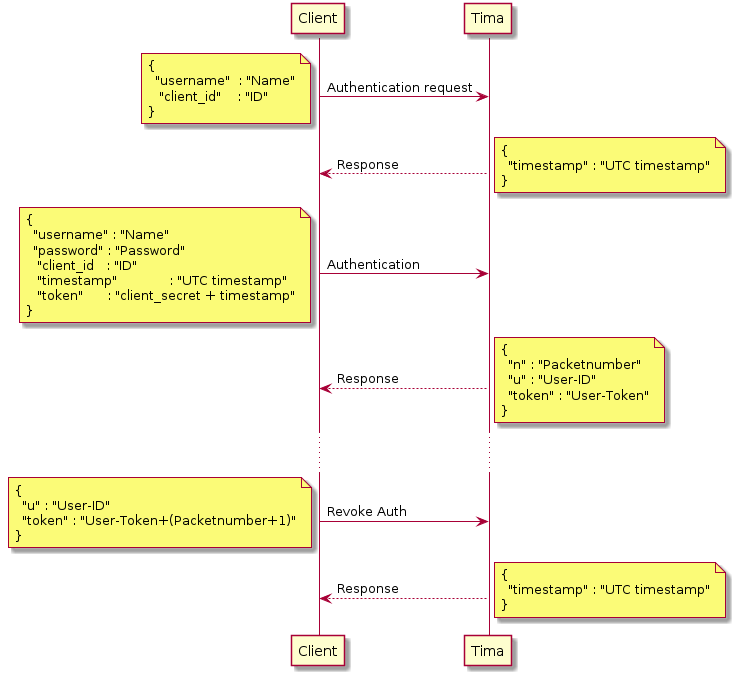
\includegraphics[width=\textwidth]{images/auth.png}
	\caption{Authentisierungsprozess}
	\label{fig:auth}
\end{figure}

In \hyperref[fig:auth]{Abbildung \ref*{fig:auth}} ist der Authentisierungsprozess schematisch dargestellt. Der Client ist dabei eine Applikation, über die sich ein Nutzer authentisieren möchte. Die Applikation verfügt zum einen über eine \code{client\_id} und über ein \code{secret}, beides von TIMA vergebene eindeutige zufällige Strings. Der Authentisierungsprozess läuft wie folgt ab:
\begin{enumerate}
	\item Eine Applikation sendet eine Anfrage an TIMA mit dem \code{username} des Nutzers und der \code{client\_id}. TIMA prüft diese beiden Werte auf Existenz und antwortet entweder mit \textbf{200} (HTTP Response Code) und dem aktuellen Zeitstempel oder mit \textbf{404}.
	\item Als nächstes sendet die Applikation die eigentliche Authentisierungsanfrage. Mit \code{username} und \code{password} des Nutzers, \code{client\_id} der Applikation, dem Zeitstempel der Antwort der letzten Anfrage und einem \code{token} das aus dem \code{secret} der Applikation und dem Zeitstempel geniert wird (SHA512).
	\item TIMA antwortet wenn die Authentisierung erfolgreich war mit \textbf{200} und den folgenden drei Werten:
	\begin{itemize}
    \item[\textbf{n}] Paketnummer - jede Anfrage einer Applikation muss diese um eins nach oben zählen. Als Wertebereich ist \code{uint32} zu benutzen.
    \item[\textbf{u}] eine eindeutige Nutzer-ID, die bei jeder Anfrage mit zusenden ist
    \item[\textbf{token}] ein zufälliger String, der bei jeder Anfrage zusammen mit der Paketnummer \code{n} in einem SHA512 Hash zu senden ist
	\end{itemize}
\end{enumerate}

Aus Kompatibilitätsgründen läuft die Paketnummer im Wertebereich \code{uint32}, also bis maximal 2147483646, und fängt nach erreichen der Maximalzahl wieder bei 0 an.

\subsection{OAI-PMH}\label{sec:oai-pmh} %TODO: Wofür?
Bei OAI-PMH (Open Archives Initiative - Protocol for Metadata Harvesting) handelt es sich um ein auf XML basierendes Protokoll zum Sammeln von Metadaten. Es wird dabei unterschieden zwischen Data Providern und Service Providern. Ein Data Provider betreibt ein oder mehrere Repositories, die OAI-PMH unterstützen um Metadaten bereitzustellen. Service Provider sammeln die Metadaten der Data Providern und bieten Mehrwertdienste an. Da TIMA ein offenes Projekt ist, liegt es nahe, derartige Projekte ebenfalls zu unterstützen.

Wir haben das OAI-PMH Protokoll implementiert um Metadaten zu den gesammelten Assoziationen bereitzustellen. Wir stellen dabei als Data Provider Metadaten zu den Wörtern und im geringen Maße zu den Nutzern bereit.
